\part{Lösungsansatz}
\label{part:solution}
\begin{frame}[fragile]{}
	\textit{Erweiternde Darstellungen räumlich und zeitlich in den Versuch integrieren}
	\pause
	\begin{itemize}
		\item Nicht sichtbare, physikalische Eigenschaften im Raum darstellen
		\begin{itemize}[topsep=-5px]
			\setlength{\itemsep}{-5px}
			\item Magnetfelder durch Feldlinien und Vektoren
			\item Stromfluss, Messwerte und ideale Kompassnadel 
		\end{itemize}
		\pause
		\item Positionierung und Stabilisierung der HoloLens nutzen		
		\item Echtzeitdaten (Messwerte) an die HoloLens übermitteln und darstellen
		\item Technische Einschränkungen beim Design berücksichtigen
	%	\begin{itemize}[topsep=-5px]
	%		\setlength{\itemsep}{-5px}
	%		\item Maßnahmen zur Vermeidung von Problemen anwenden
	%		\item Angepasstes Design
	%		\item Vorgefertigte Objekte nutzen
	%	\end{itemize}
		\item Anpassung von realen Objekten, um Integration mit der Anwendung zu verbessern
	\end{itemize}
\end{frame}

\begin{frame}[fragile]{Design}
	\vspace{-10px}
	\begin{minipage}{0.25\textwidth}
		{\setstretch{1.0}
			\begin{itemize}[itemsep=1mm]
				\item Feldlinien
				\item Skala
				\item Auslenkung
				\item Stromrichtung
				\item Plus \& Minus
				\item Messwerte
			\end{itemize}
		}
	\end{minipage}
	\begin{minipage}{0.7\textwidth}
		\centering
		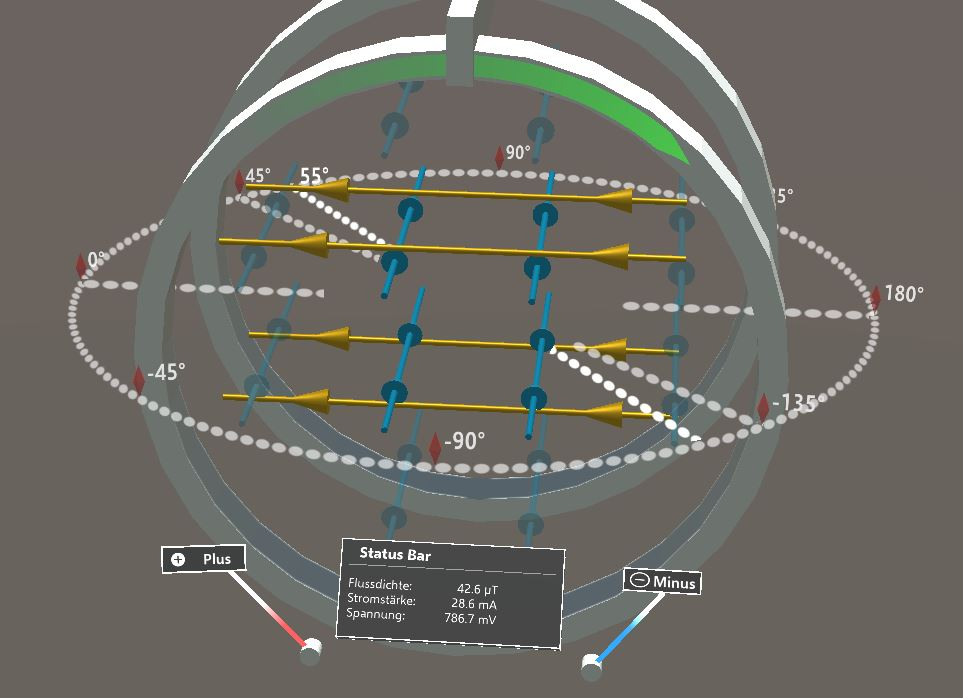
\includegraphics[width=0.95\textwidth]{images/unity/overview.jpg}\\
		\scriptsize Darstellungen in der Entwicklungsumgebung (Unity). Auflösung und Qualitätseinstellungen entsprechen den Werten auf der HoloLens.
	\end{minipage}
\end{frame}

\begin{frame}[fragile]{Design}
\vspace{-10px}
\begin{minipage}[t]{\textwidth}
	{\setstretch{1.0}
		\begin{itemize}[itemsep=1mm]
			\item Platzsparendes Design, um Screenspace zu nutzen und in FoV-Grenzen zu bleiben, außerdem günstig für Stabilisation
			\item Minimal notwendige Anzahl Feldlinien bzw. Vektoren
			\item Nutzung konzipiert für: 1,3 m Abstand und $0^\circ$ bis -$35^\circ$ Winkel (vertikal)
		\end{itemize}
	}
\end{minipage}


\begin{minipage}{0.6\textwidth}
	{\setstretch{1.0}
	\begin{itemize}[itemsep=1mm]
		\item Begrenzungen über Transparenz
		\item Objekte orientieren sich an Nutzerposition
		\item Bekannte Darstellungsmodelle
		\item Interaktion über Klicker/Gesten/Sprache
	\end{itemize}
	}
\end{minipage}
\begin{minipage}{0.35\textwidth}
	\centering
	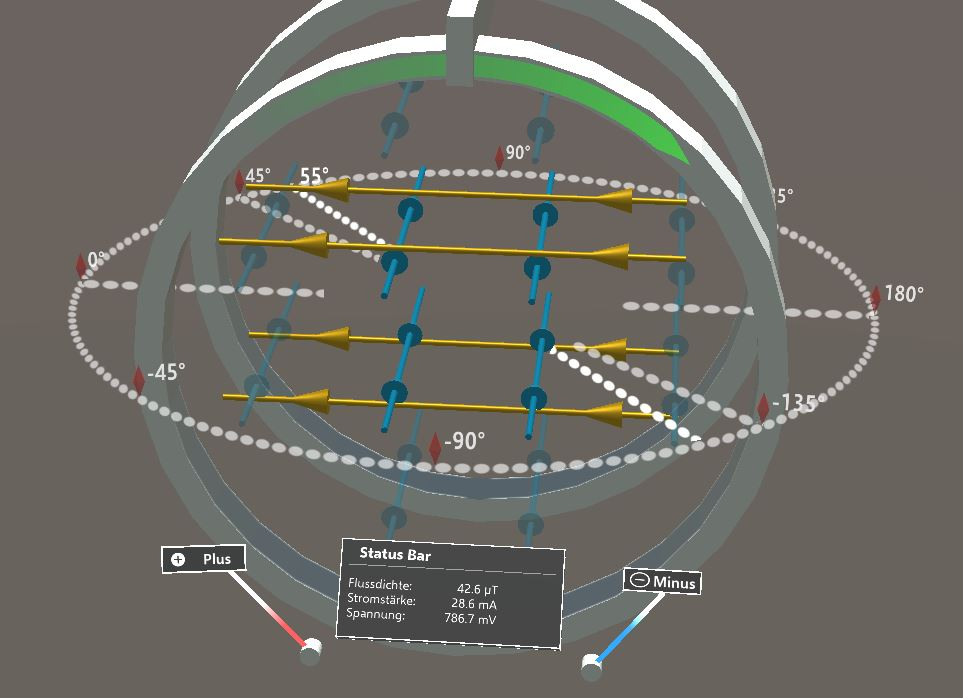
\includegraphics[width=0.95\textwidth]{images/unity/overview.jpg}\\
\end{minipage}
\end{frame}

\begin{frame}[fragile]{}
\pause
\begin{figure}
	\vspace{-10px}
	\centering
	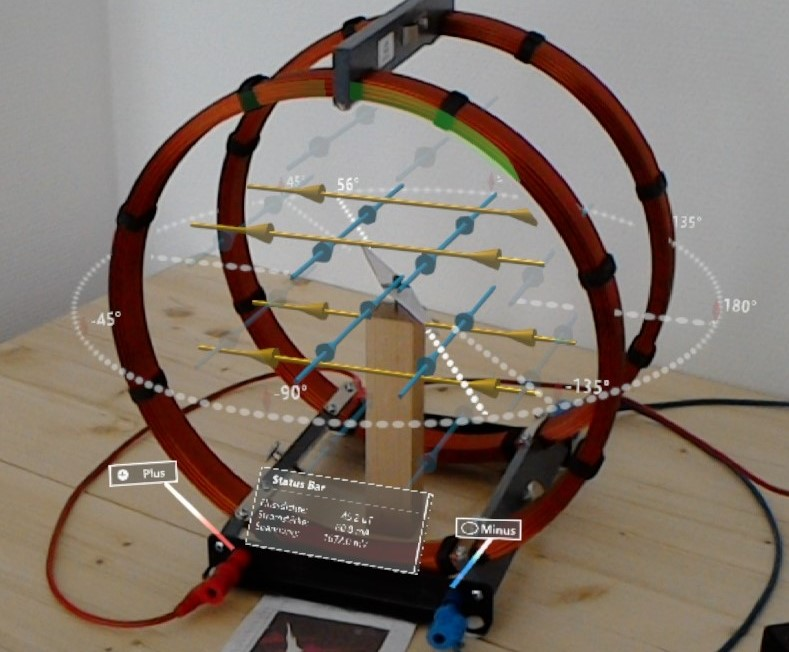
\includegraphics[width=0.7\textwidth]{images/HL/fieldlines_cut.jpg}\\
	\scriptsize Screenshot von der HoloLens mit Feldliniendarstellung.
\end{figure}
\end{frame}

\begin{frame}[fragile]{}
\begin{figure}
	\vspace{-10px}
	\centering
	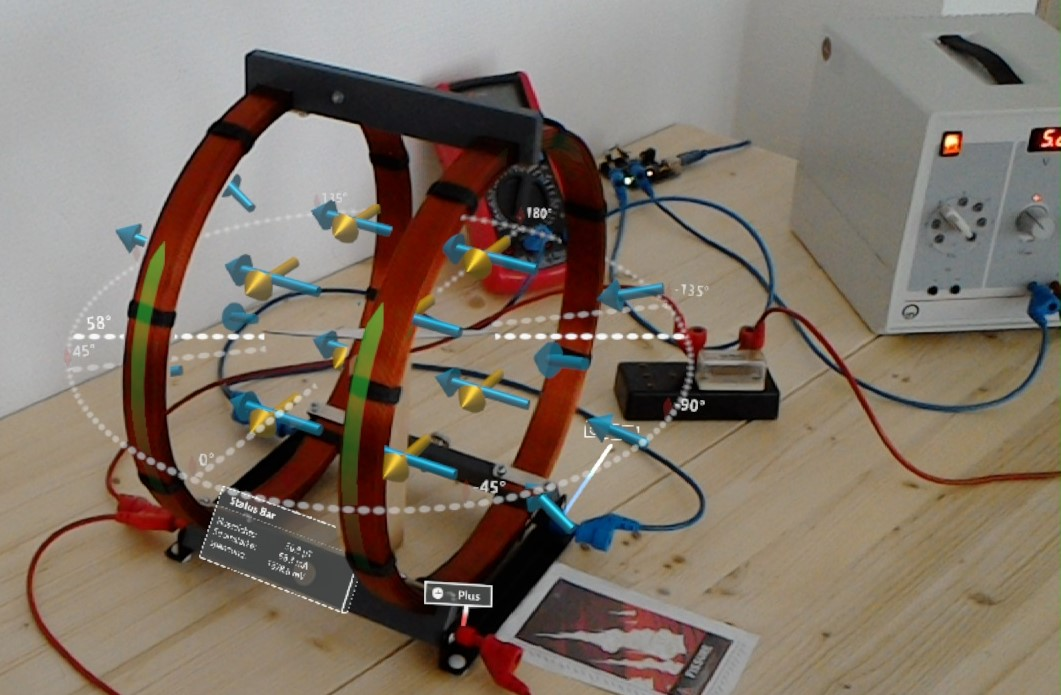
\includegraphics[width=0.85\textwidth]{images/HL/Vektoren.jpg}\\
	\vspace{0.3cm}	
	\scriptsize Screenshot von der HoloLens mit Vektordarstellung.
\end{figure}
\end{frame}

\begin{frame}[fragile]{}
\begin{figure}
	\vspace{-10px}
	\centering
	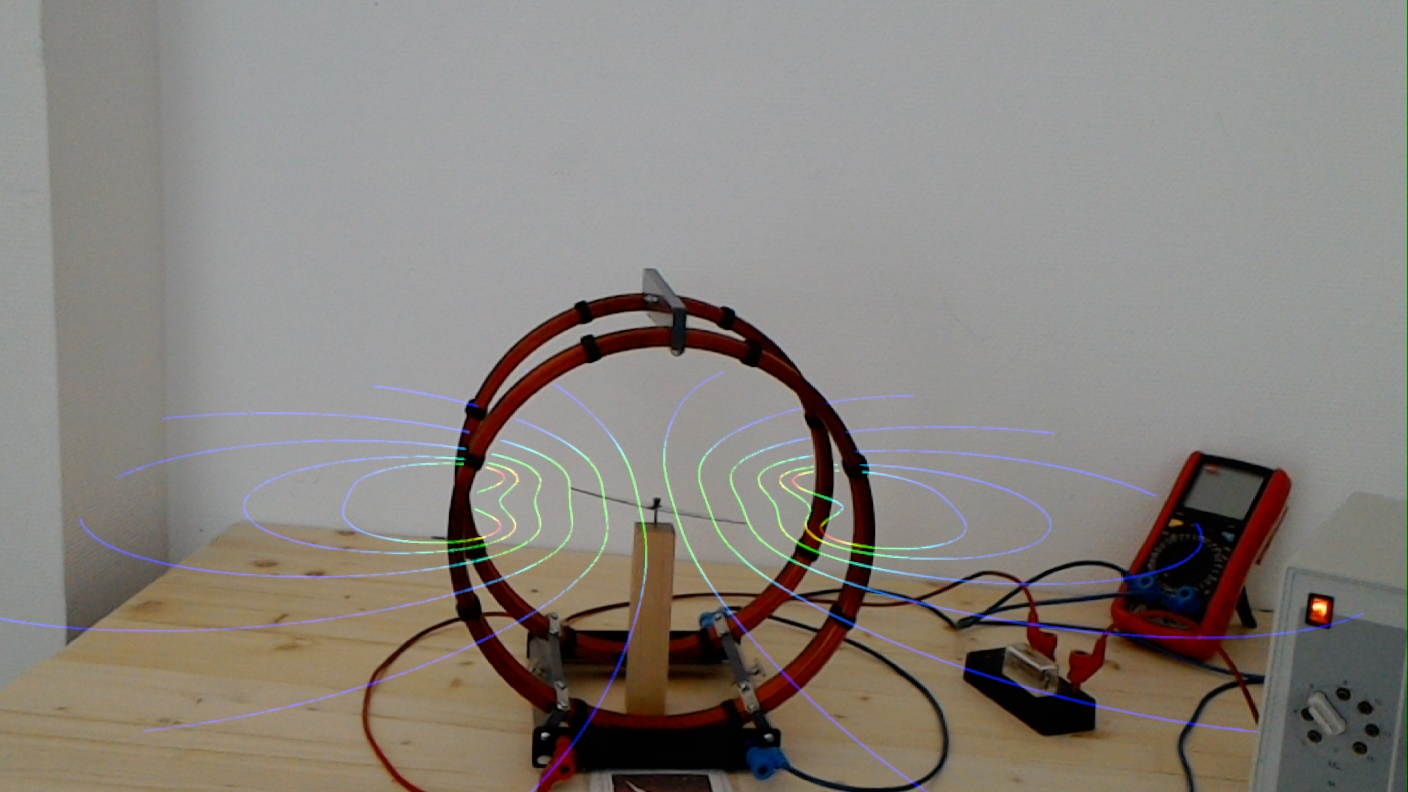
\includegraphics[width=0.95\textwidth]{images/HL/simulation.jpg}\\
	\vspace{0.3cm}
	\scriptsize Screenshot von der HoloLens mit Darstellung von Simulationsdaten.
\end{figure}
\end{frame}

\begin{frame}[fragile]{Near Plane Fading}
\begin{figure}
	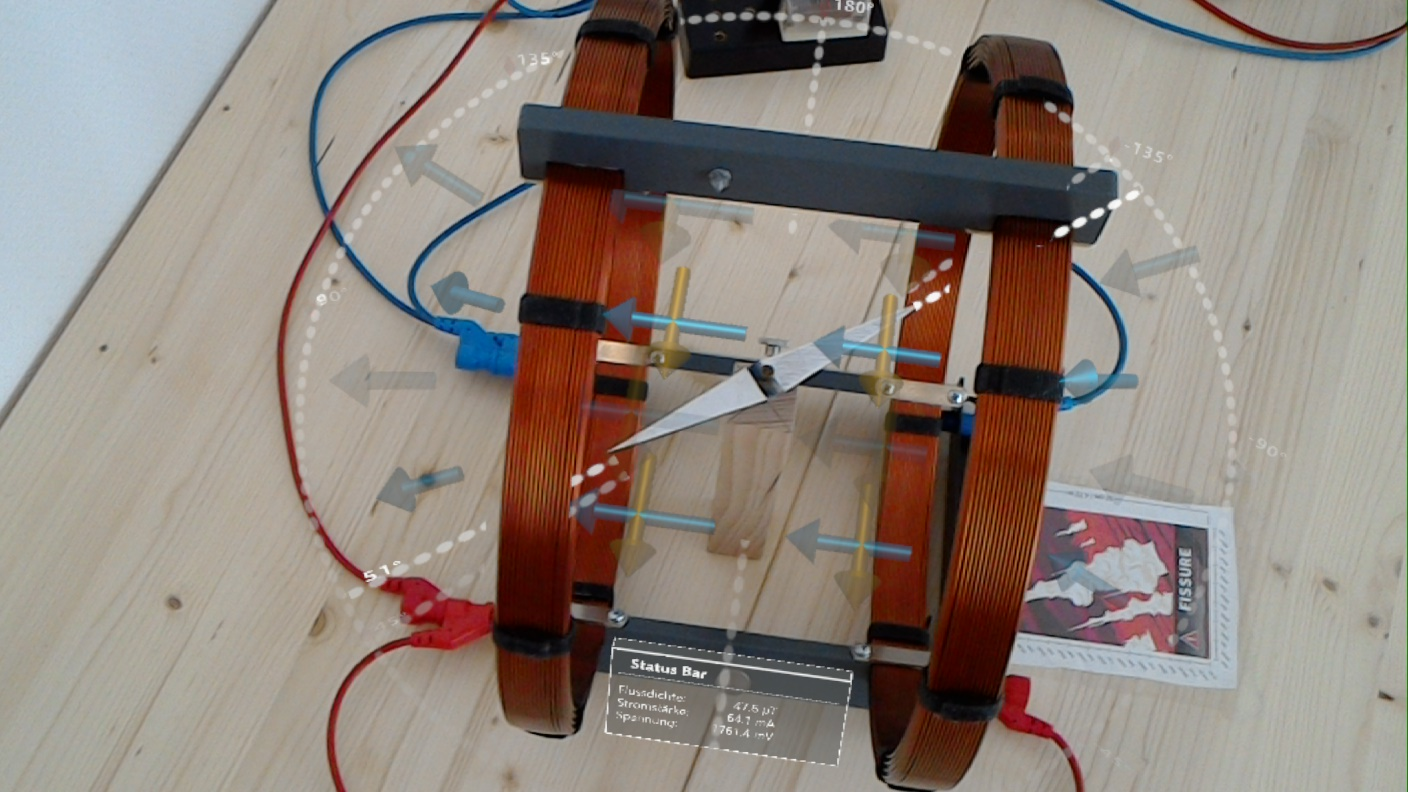
\includegraphics[width=0.8\textwidth]{images/HL/compass.jpg}\\
	\vspace{0.3cm}
	\scriptsize Dicht liegende Objekte werden ausgeblendet. Kompassnadel ist weiß überklebt, damit sie besser zu erkennen ist.
\end{figure}
\end{frame}
